\chapter{Model training}
\label{chap:tuning}

In this chapter, we are going to describe our process of developing
the statistical post-editing models. We will take a closer look at the feature selection
methods we have experimented with, the task of model selection and parameter
tuning and also the methods of evaluation we used during the tuning.
The experiment results reported in this chapter are only for the separate
classifier components, results of the evaluation of the whole MLFix systems
are provided in the following chapter. The evaluation presented in this chapter
is done on a word level, because it reflects our definition of an extracted instance.

In this chapter, we will cover following two classification tasks: the identification
of the incorrect instances (words from the MT output with incorrect surface form)
and the prediction of the new morphological categories for the incorrect instances.

\section{Automatic error classification}

%data rep - # of features
%cv method
%baseline

We have found that not only during task specification but even during model training,
the task of identifying morphologically incorrect words in the text is more difficult
the task of assigning the new morphological categories. We have faced several issues
during training which we will describe in more detail in the following subsections.

\subsection{Unbalanced data problem}

In this task, we face the problem of the binary classification, where we decided
to assign value 0 to the instances that we consider correct and value 1 to the
instances that need to be corrected. The process of assigning these values to the
extracted training instances was described in the previous chapter. 

For the model evaluation, we defined a baseline classifier, which assigned the 0 value
to each instance, therefore marking all of the MT output as already correct.
This baseline already achieved accuracy larger than 95\%, because, as we have already shown,
only a small portion of our
training instances has been marked as incorrect by our heuristic.
This became a several issue since most of the machine learning method use accuracy during
the process of searching for the best hypothesis. On the other hand, it is the minority
class, that is our target during the error classification.

There are several methods that can be used to solve this problem: creating syntetic
training data by resampling instances with our minority class or removing some instances
belonging to the dominating class, weighting of the training instances, modification of the
cost function. The manipulation with the training data (upsampling, downsampling) is the easieast method,
however, the more it modifies the distribution of the classes over the training data, the worse is the final
performance of the classifier on the real-life data. Still, the idea of modifying the distribution
of our training data is worth considering.

We inspired ourselves in the work of Jia\cite{biblio:ZaPoHiddenMarkov2009}, where they face similar
classification task. During training, they filtered their training corpus using only around 5\% of
the sentences, because only those were the ones that contained grammatical errors.

In our case, when we look at the results produced by the Oracle classifier, we can see that at least
two-thirds of the MT sentences have not been modified (and would not be due to our method of marking
the incorrect instances). These \equo{correct} (ignored by the Oracle) sentences are still part of
our original training data. Therefore, to balance our data, we have decided to use only the training
instances from the sentences where at least one word was marked as incorrect. This way, we were
able to increase the portion of the minority class up to 10\%.

\todo{kam s popisem metrik?}

For this reason
we decided to use precision and recall based metrics during the model tuning with
our main focus turned to maximising the model precision rather than the recall,
because we think it is more preferable to miss some of the incorrect instances than falsely mark
instances which are actually correct.

For the purposes of evaluation we compute \pojem{precision} by a widely used formula:
$precision = TP / (TP + FP)$
where TP stands for \pojem{true positives}, in our case instances which were
assigned same value as the \pojem{true prediction} and different value than the \pojem{baseline},
and FP stads for \pojem{false positives}, the instances which were assigned value
different from both \pojem{true prediction} and the \pojem{baseline}.

Similarly, we define \pojem{recall} with a following formula:
$recall = TP / (TP + FN)$
where FN stands for \pojem{false negatives}, the instances which were assigned value
different from the \pojem{true prediction} and equal to the \pojem{baseline}.
This specific definition of TP, FP and FN is similar to the standard interpretation
of these terms due to the choice of our baseline. However, it will be important
during evaluation of the second classification task, the prediction of new morphological
categories.

Our training process can be separated into two stages: in the first stage, we
focused on choosing a suitable machine learning method, we chose the most promising
one and in the second stage we tried to further increasing the performance of model
based on the chosen method by experimenting with various methods of feature filtering.
We will take a closer look on both stages in the following subsections.

\subsection{Machine learning method comparison}

There are many machine learning methods that support binary classification, so we
decided to only compare a limited subset of the available methods that are implemented
in the Scikit-Learn framework. For each classifier we tried several hyperparameter
settings to observe the changes in the classifier behaviour. However, we have maded only
a rough examination of the hyperparameter configuration due to the number of observed
methods. In this stage, the goal was not to train the best possible classifier but
eliminate those, that are not suitable for the task.

We tried to measure the performance of the classifiers on several datasets. We used
the Autodesk dataset, WMT10 data, dataset extracted from the lingea logfiles and
WMT16 newstest dataset translated, one with the Chimera system and
one translated with the experimental neural network machine translation system (NMT)
provided by the University of Edinburgh\todo{no ref, nezminovat?}. For each dataset a counterpart
created by substitution of the reference sentences by the Depfix output was also created
to additionally measure the performance on the \equo{syntetic} data.

For the purposes of the coarse evaluation we used each dataset separately for both training
and testing of the classifers, by performing one-against-the-rest 10-fold jackknife sampling.
Therefore the performance measured in this stage should be considered only as an in-domain
performance for a specific MT system.

We have compared the following methods: logistic regression, ridge regression classifier,
random forests, extremely randomized trees and support vector machines classifier.
In the\todo{ref}, we can see the comparison of the performance of various classifiers based
on the F1-measure metric. %okec

% todo: src, nosrc
% init features: 1364
% init features: 682
% napsat do feat filtering
% best + avg


% The summary of precision-recall performance of each trained classifier is shown
%in table\todo{ref}.
%TODO okec


\subsection{Feature filtering}

%TODO: feature representation - vectorized dicts, binary features


\section{Prediction of new categories}

The second classification problem was predicting the correct morphological category for
the words that were marked as incorrect. Because we are using the Interset representation
of the morphological features we have several possibilities, how to handle this task such
as:
\begin{enumerate}
    \item predict each category separately,
    \item concatenate the features and treat them as a single prediction target,
    \item use the methods that support multitask classification,
\end{enumerate}

With the first option, the biggest issue is determining the order in which the classifiers
should be aplied mainly if we also want to include the current node morphological features
into our model's feature set. The second approach eliminates this problem by predicting the
values simultaneously. This can, however, quite easily expand the set of the predicted values,
which will usually lead to an increased data sparsity. This can be a big problem as we have
already shown that the amount of data, available for the post-editing task (mainly the post-edited
data) can be quite low. The third option combines the first two by training an estimator
which handles multiple joint classification tasks, one for each morphological category. The
Scikit-Learn toolkit provides several classifiers which support this option.

Before jumping straight into training our classifier, it is important to examine what morphological
changes are made in our training data, how frequent they are and how can they affect the resulting
surface form generation. We can, for instance, predict new values of the \samp{punctype} category,
but it is almost certain that it will not affect the resulting wordform of any of the words
classified as incorrect, because this category is related strictly to punctuation. There are
of course less obvious examples and some categories, while being relevant for one target language
can be pointless in another.

For this reason we made a frequency analysis of the changes encountered
in our data, shown in the figure\Fref{iset-barplot}. We can see that most of the time, only the grammatical
case was modified (more than 50\% of the instances for the Depfix-based datasets and more than 40\% of the instances for
the normal datasets). Other changes were a lot less frequent (less than 10\% of the modified instances), however,
we decided that it still might be worthwhile to try at least predicting grammatical number and gender.

\subsection{Machine Learning method comparison}

In the end, we decided to train three models: one predicting case only (C), one predicting case and number (CN),
and one predicting case, number and gender (CNG). We used same datasets as in the previous task, however, this
time we have used only feature vectors of the instances that were marked as incorrect in our training data. Because
our predictors will only be classifying the incorrect instances, training them on the whole dataset would only create
unnecesary bias.

Again, we had to decide which ML method should we use for this task. We have ran similar set of classifiers with similar
hyperparameters as in the error classification task to get a rough idea about their capabilities. The metrics we have used
are also the same. The results are shown in~\Fref{cats-draft}. We can see, that even without any sophisticated parameter
tuning or feature filtering, the classifiers perform quite well. We can also notice that in most of the cases, the ensemble
methods (random forests, extremely randomized trees) performed slightly better than the rest. Therefore we have decided
to pick these methods for further experiments.

\begin{figure}
\centering
  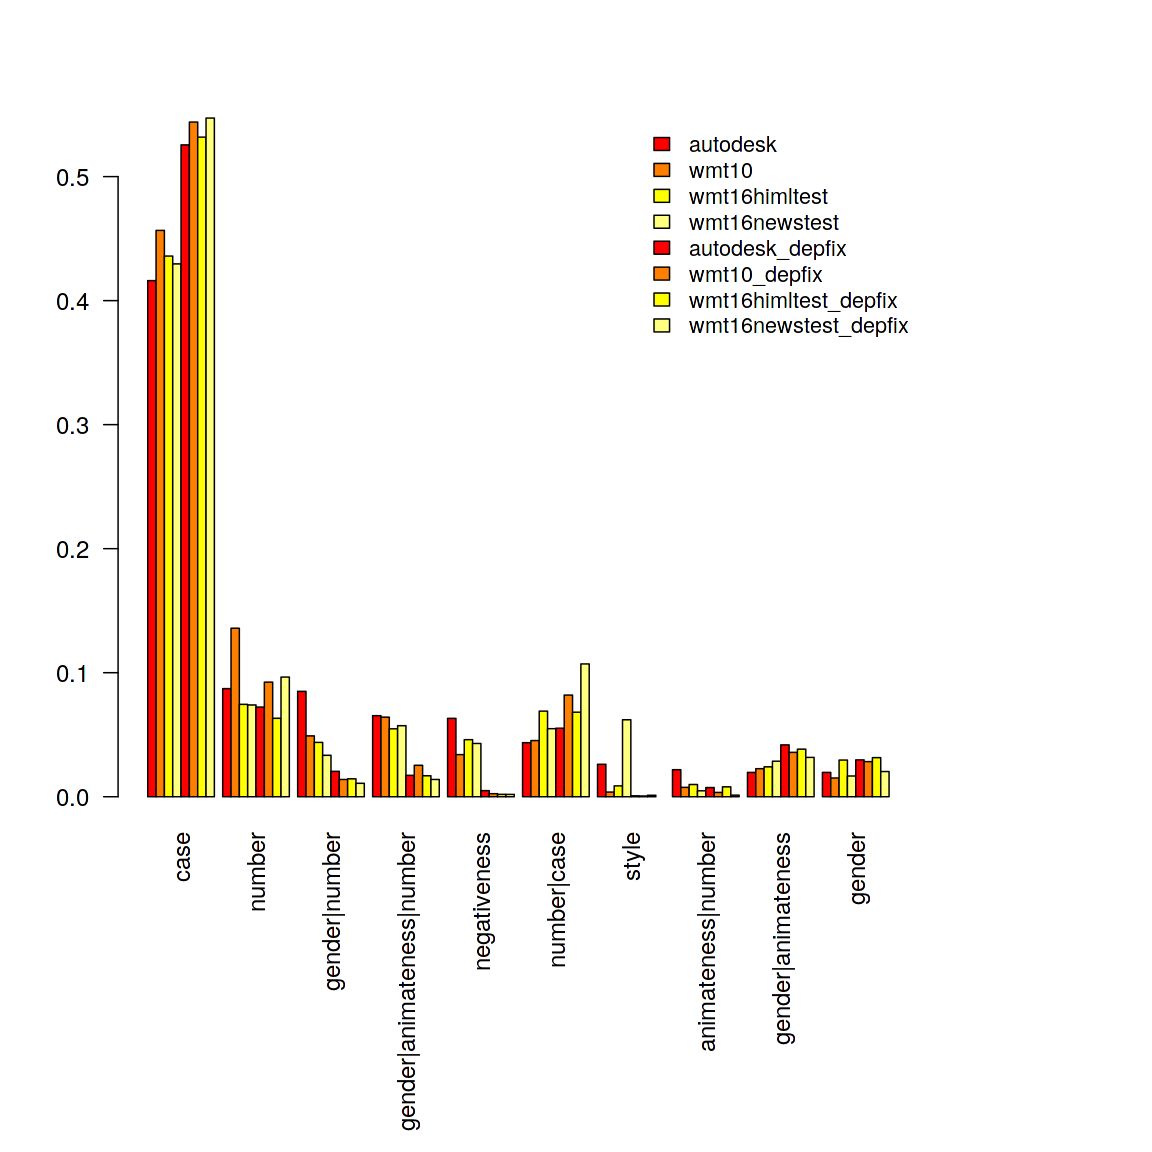
\includegraphics[scale=0.7]{iset}
  \caption{
    Frequency of the most changed Interset categories, grouped by a datasets. Categories containing
    "\textbar" symbol (e.g. gender\textbar{}number) represent changes made simultaneously.
}
  \label{iset-barplot}
\end{figure}

% with source
\begin{figure}
\centering
  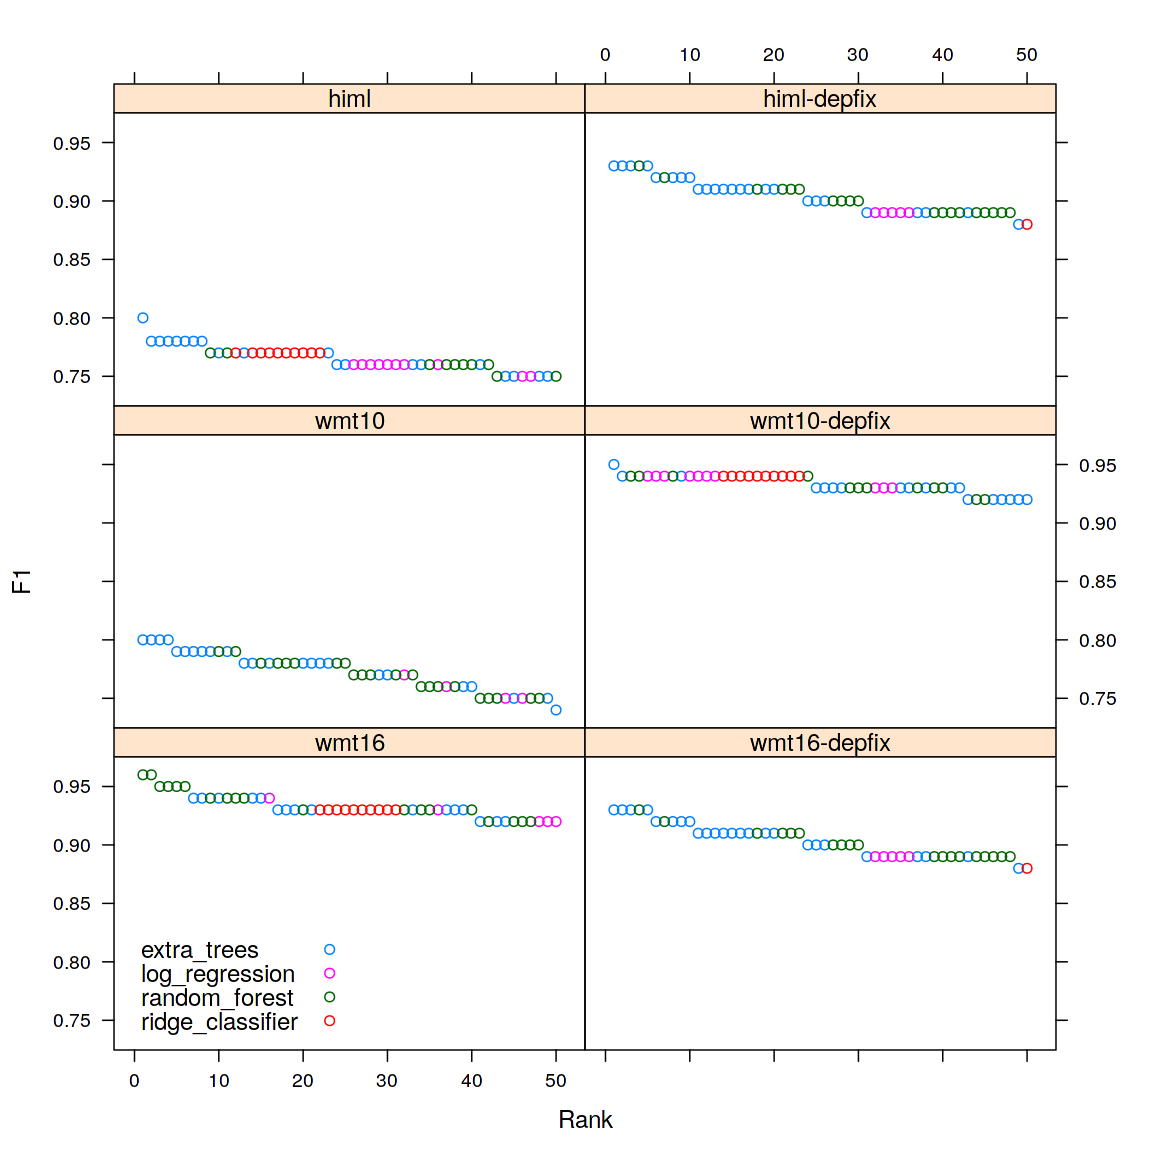
\includegraphics[scale=0.7]{cat-class}
  \caption{
    Overview of the classifier performance. We have tried several variations of the hyperparameters
for each classifier. The classifiers are ordered from the best to the worst. Only top 50 classifiers
are shown for each dataset.
}
  \label{cats-draft}
\end{figure}


